%#!platex ./report.tex

\chapter{$B7k2L(B}
 \section{Passive$B$N7k2L(B}
   \subsection{$B@h9T8&5f<jK!(B\cite{torben2009systematic}$B$H$NHf3S(B}
     $BK\8&5f<jK!$H@h9T8&5f$GMQ$$$i$l$F$$$?8DBNI>2A;XI8$H$NHf3S$r0J2<$N(B
     $B?^(B\ref{Tsuishi_Rerative1}, $B?^(B\ref{Tsuishi_Rerative2}$B$K<($9(B. 

%subfigure $B$rF~$l$k$H$-$K2~9T$9$k$H!"<B:]$NJ8>O$G$b2~9T$,H?1G$5$l!"2#$KJB$P$J$/$J$k$k$N$GCm0U(B
     \begin{figure}[H]
       \begin{subfigure}{0.5\columnwidth}
         \centering
         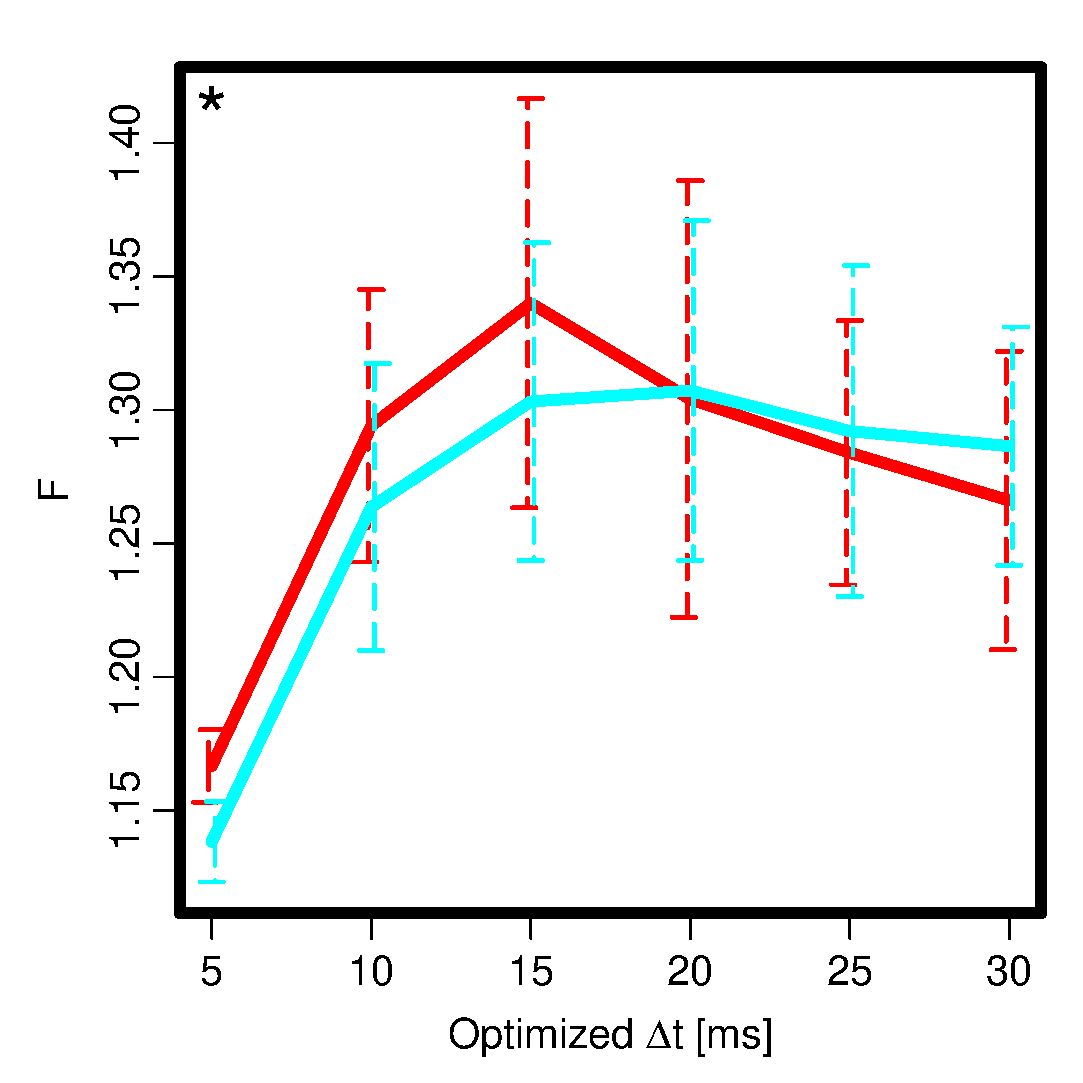
\includegraphics[width=0.8\columnwidth]{./Images_Result/Tsuishi_Rerative_F.eps} 
         \caption{F}
         \label{Tsuishi_Rerative_F}
       \end{subfigure}
       \begin{subfigure}{0.5\columnwidth}
         \centering
         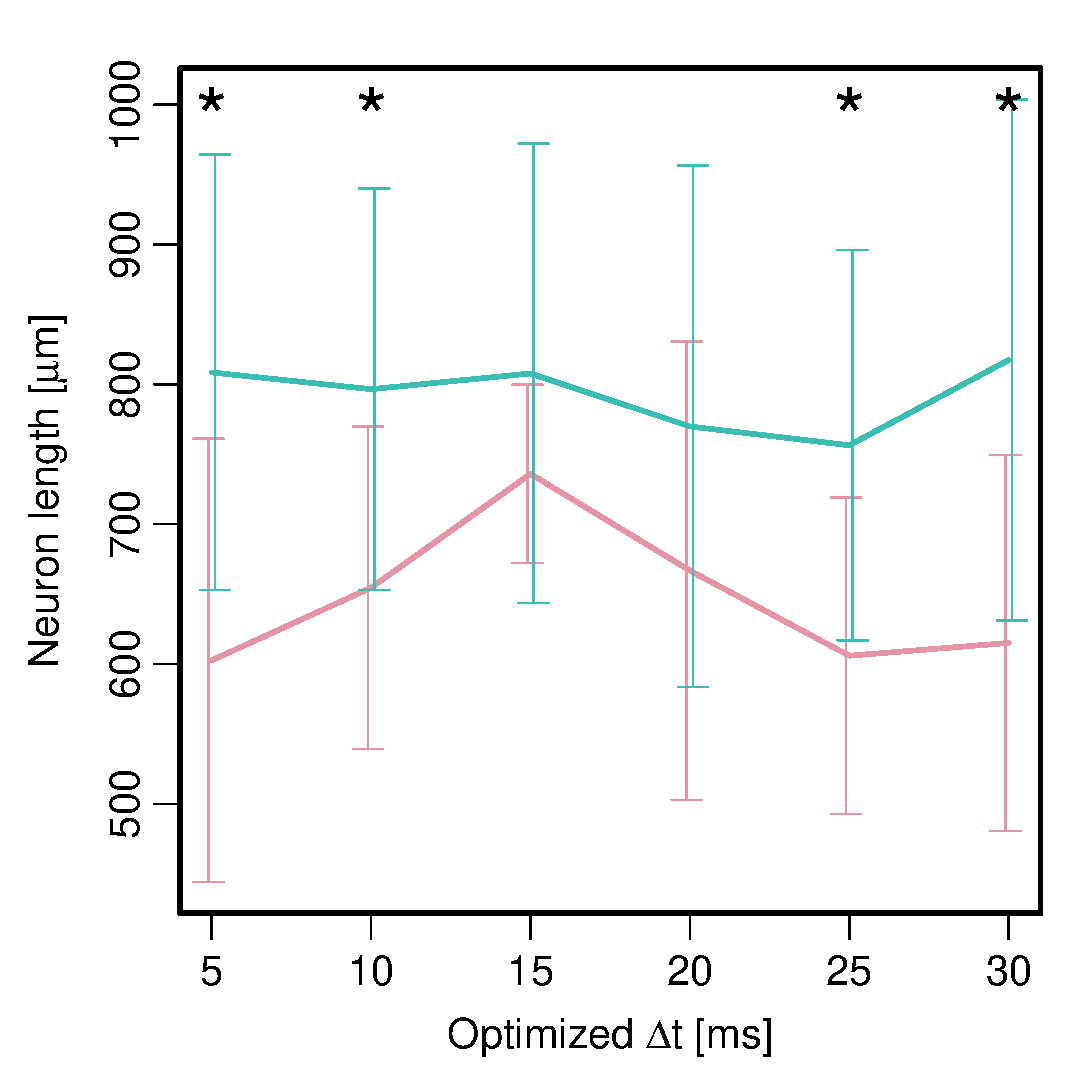
\includegraphics[width=0.8\columnwidth]{./Images_Result/Tsuishi_Rerative_TREE_length.eps} 
         \caption{$BD9$5(B}
         \label{Tsuishi_Rerative_length}
       \end{subfigure}

       \begin{subfigure}{0.5\columnwidth}
         \centering
         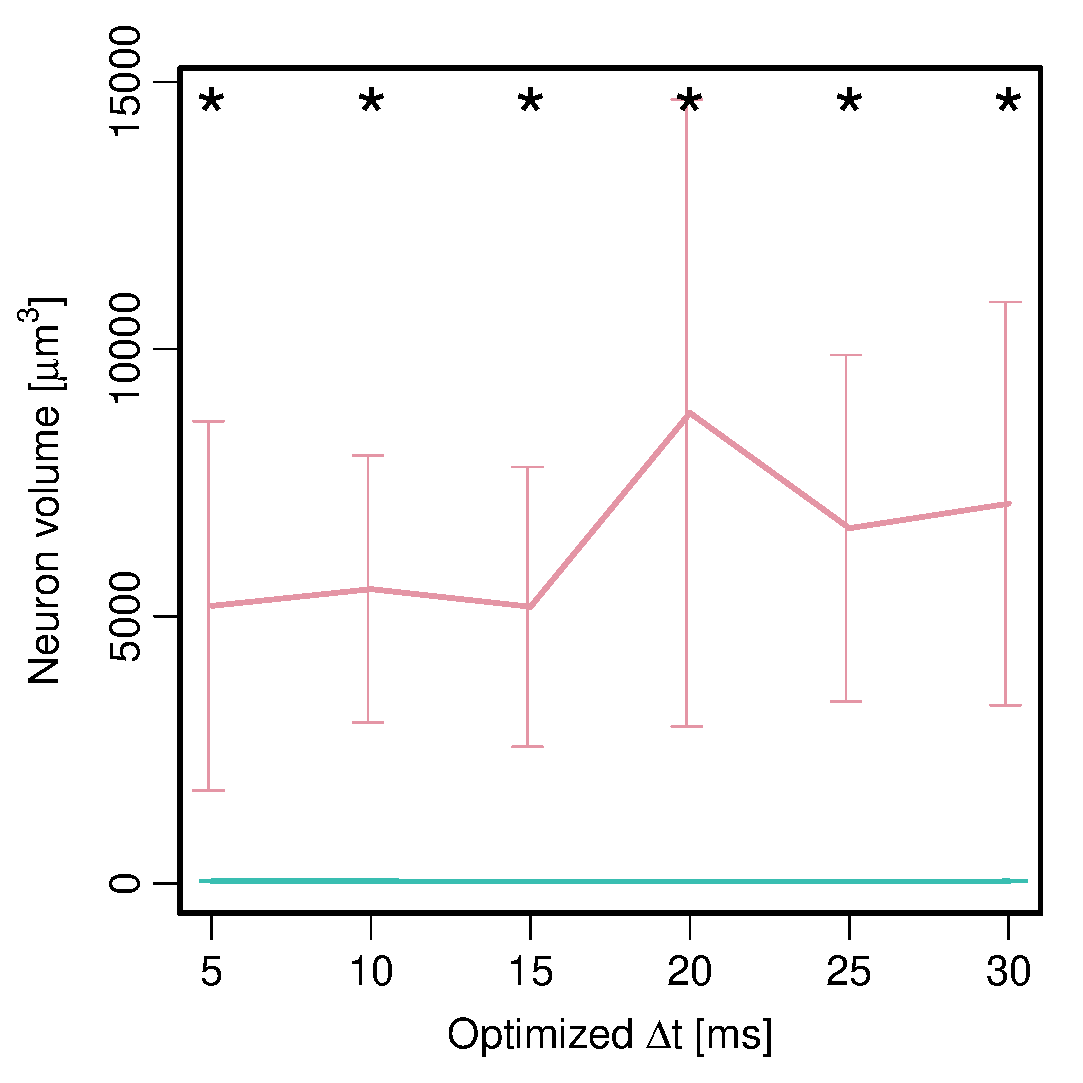
\includegraphics[width=0.8\columnwidth]{./Images_Result/Tsuishi_Rerative_TREE_volume.eps} 
         \caption{$BBN@Q(B}
         \label{Tsuishi_Rerative_volume}
       \end{subfigure}
       \begin{subfigure}{0.5\columnwidth}
         \centering
         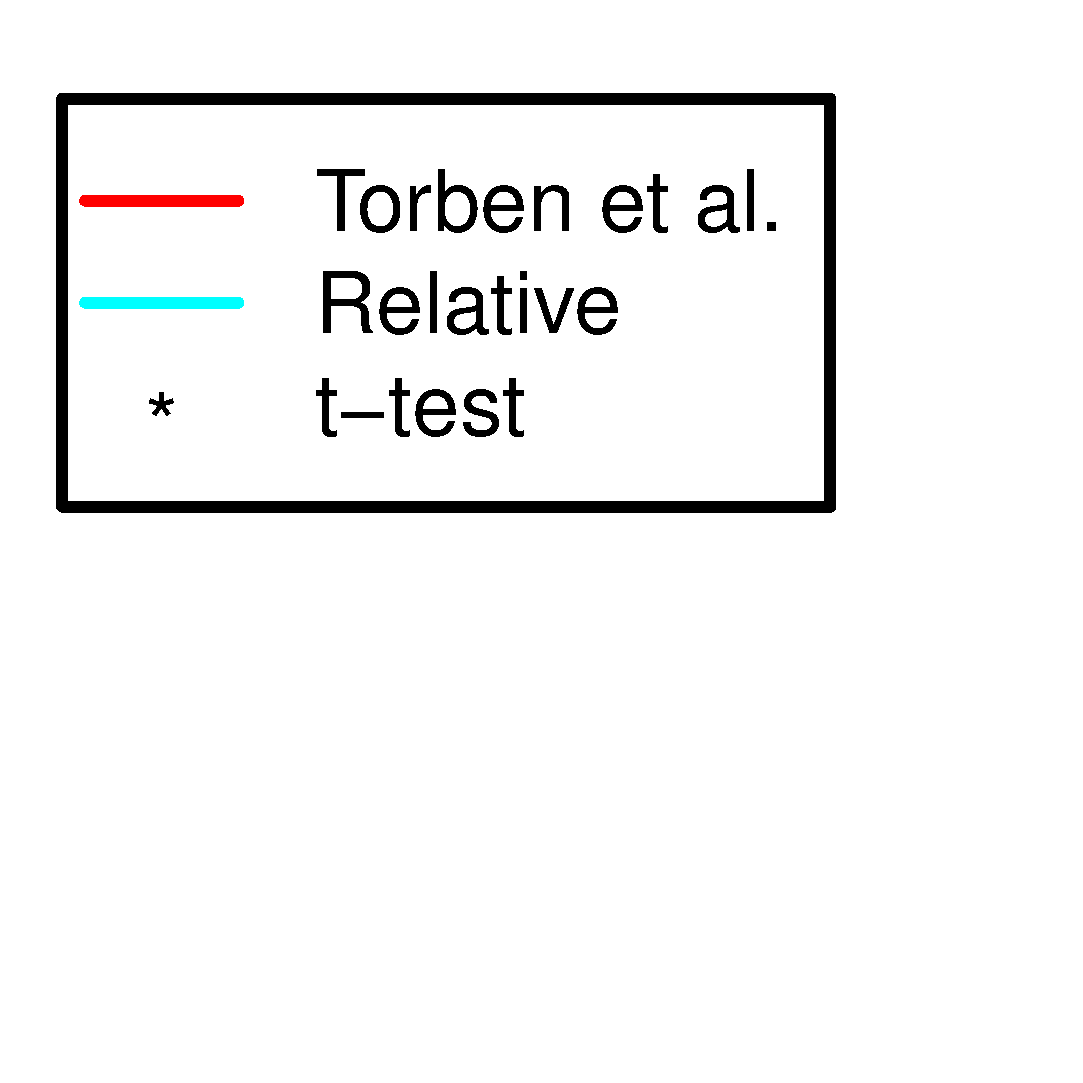
\includegraphics[width=0.5\columnwidth]{./Images_Result/Tsuishi_Rerative_legend.eps} 
       \end{subfigure}

       \caption{$B@h9T8&5f<jK!$H$NHf3S(B1}
       \label{Tsuishi_Rerative1}
     \end{figure}

     \begin{figure}[H]
       \begin{subfigure}{0.5\columnwidth}
         \centering
         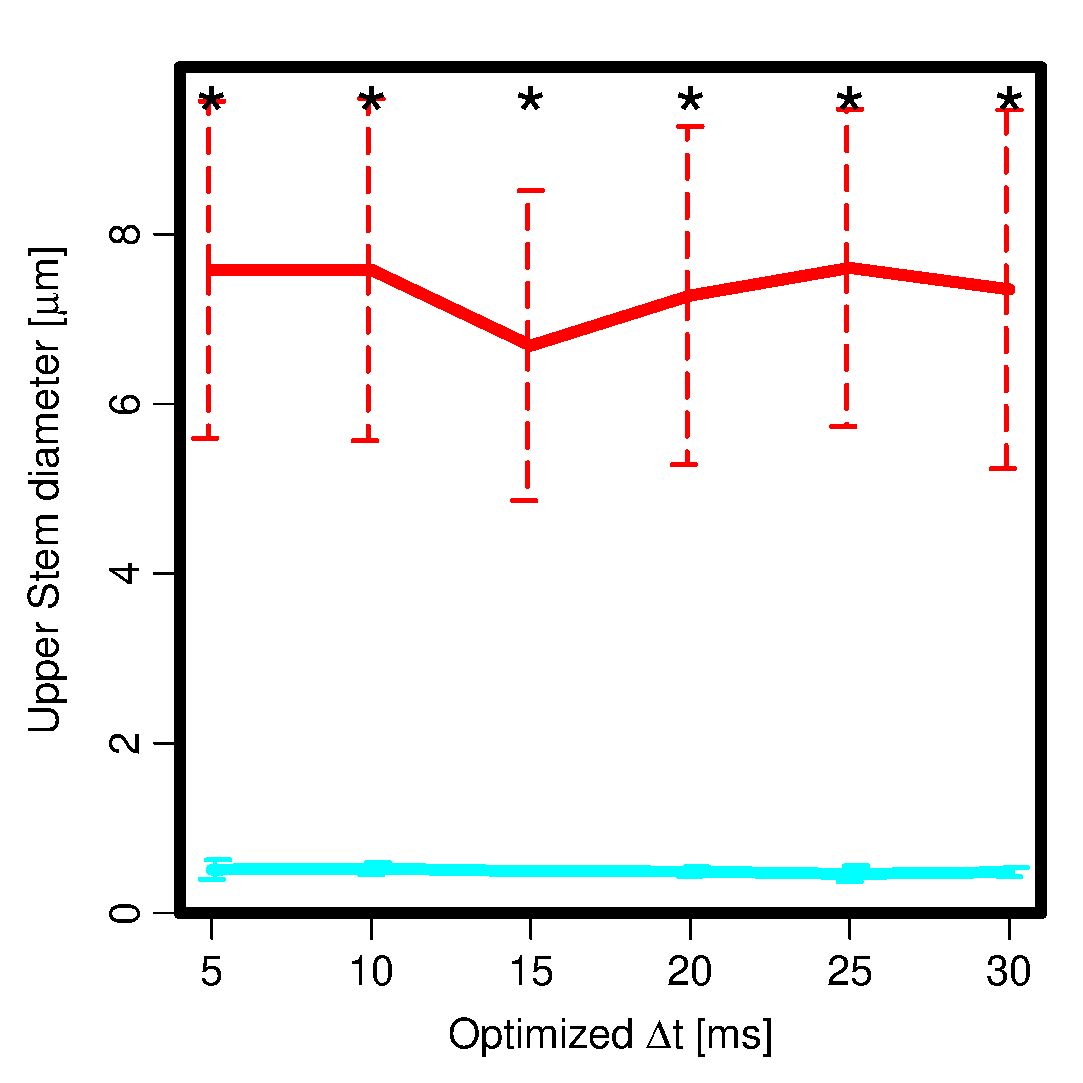
\includegraphics[width=0.8\columnwidth]{./Images_Result/Tsuishi_Rerative_Upper_Diam.eps} 
         \caption{Upper Dendrite$B$ND>7B(B}
         \label{Tsuishi_Rerative_Upper_Diam}
       \end{subfigure}
       \begin{subfigure}{0.5\columnwidth}
         \centering
         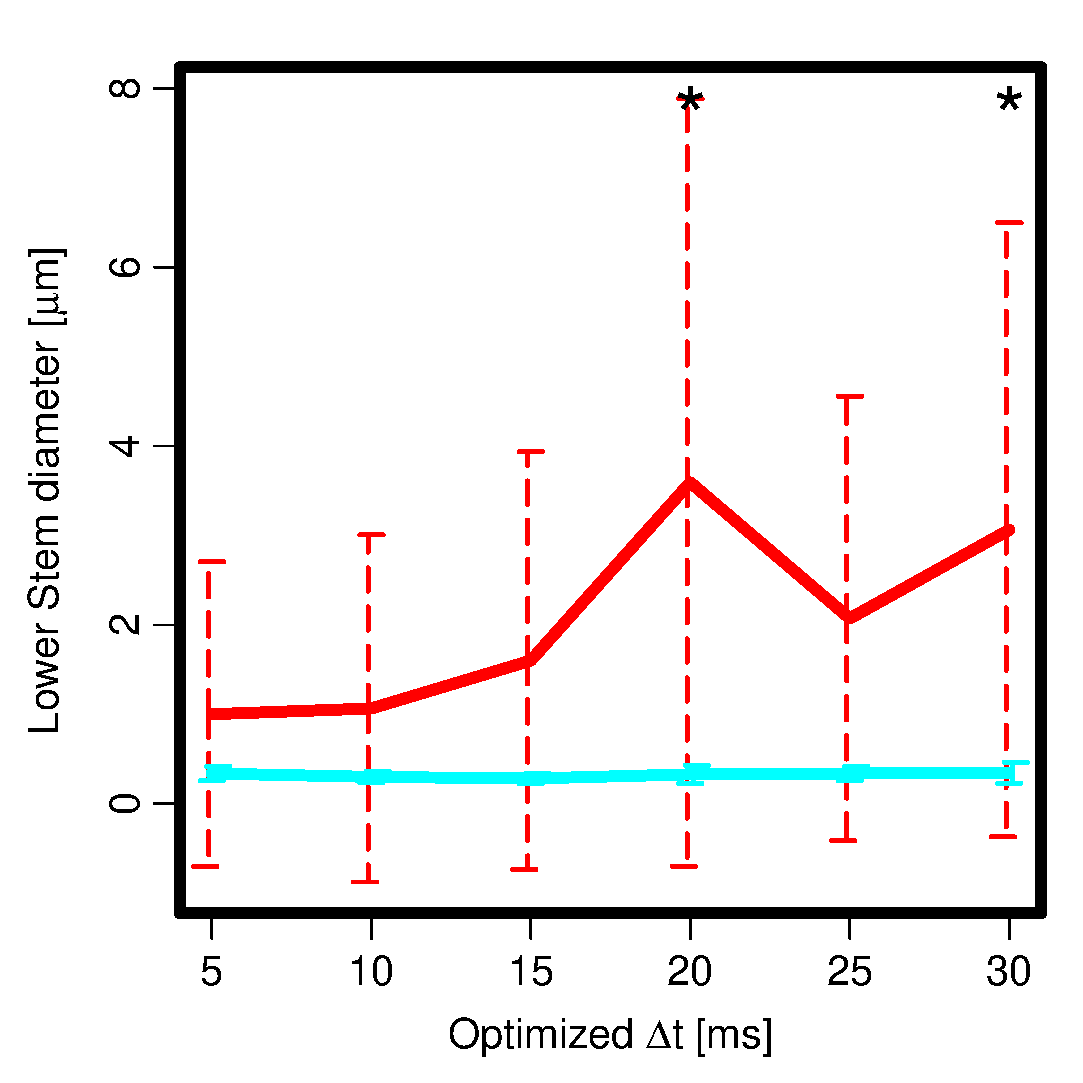
\includegraphics[width=0.8\columnwidth]{./Images_Result/Tsuishi_Rerative_Lower_Diam.eps} 
         \caption{Lower Dendrite$B$ND>7B(B}
         \label{Tsuishi_Rerative_Lower_Diam}
       \end{subfigure}
       %% \begin{subfigure}{0.3\columnwidth}
       %%   \centering
       %%   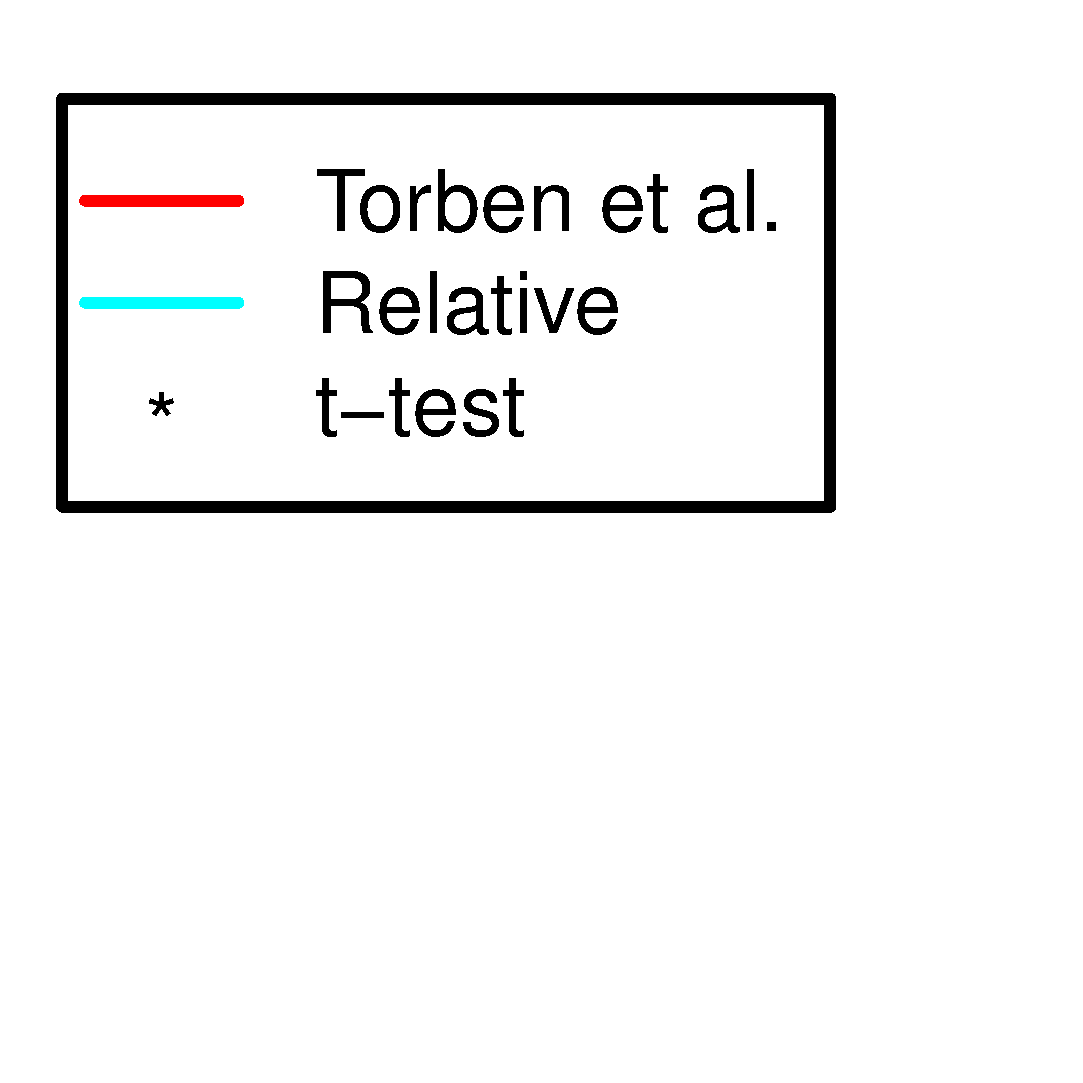
\includegraphics[width=\columnwidth]{./Images_Result/Tsuishi_Rerative_legend.eps} 
       %% \end{subfigure}
       \caption{$B@h9T8&5f<jK!$H$NHf3S(B2}
       \label{Tsuishi_Rerative2}
     \end{figure}
     $B?^Cf2<It$N@10u(B(${\star}$)$B$O%&%'%k%A$N(Bt$B8!Dj(B(${\alpha} = 0.05$)$B$rMQ$$$F@h9T8&5f<jK!(B(Torben et al)$B$HK\8&5f<jK!(B(Rerative)$B$NJ?6QCM$r(B
     $BHf3S$7(B, $BM-0Y:9$,$"$C$?$3$H$r<($9(B. 
     $B?^(B\ref{Tsuishi_Rerative_F}$B$H?^(B\ref{Tsuishi_Rerative_volume}$B$+$i$o$+$k$h$&$K(B2$B$D$N<jK!$N4V$G5!G=@-(B$F$$B$NCM$O$"$^$j:9$O8+$i$l$J$$$,(B
     $BBN@Q$OL@$i$+$K>.$5$/$J$C$F$$$k$3$H$,$o$+$k(B. 
     $B$^$?(B, 2$B$D$N<jK!$G@8@.$5$l$??@7P:YK&$NNc$r?^(B\ref{passive_morphos}$B$K<($9(B. 
     \begin{figure}[H]
       \begin{subfigure}{0.5\columnwidth}
         \centering
         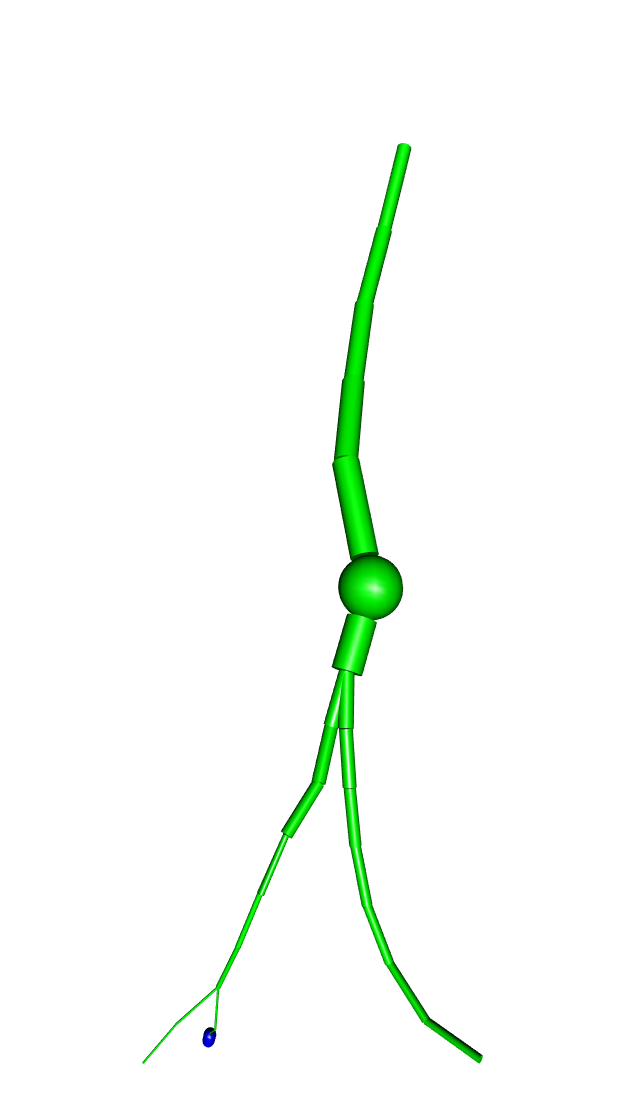
\includegraphics[width=0.7\columnwidth]{./Images_Result/alfa_sample.png} 
         \caption{$B@h9T8&5f$N<jK!$G:n@.$7$??@7P:YK&7ABV(B}
         \label{Tsuishi_sampel}
       \end{subfigure}
       \begin{subfigure}{0.5\columnwidth}
         \centering
         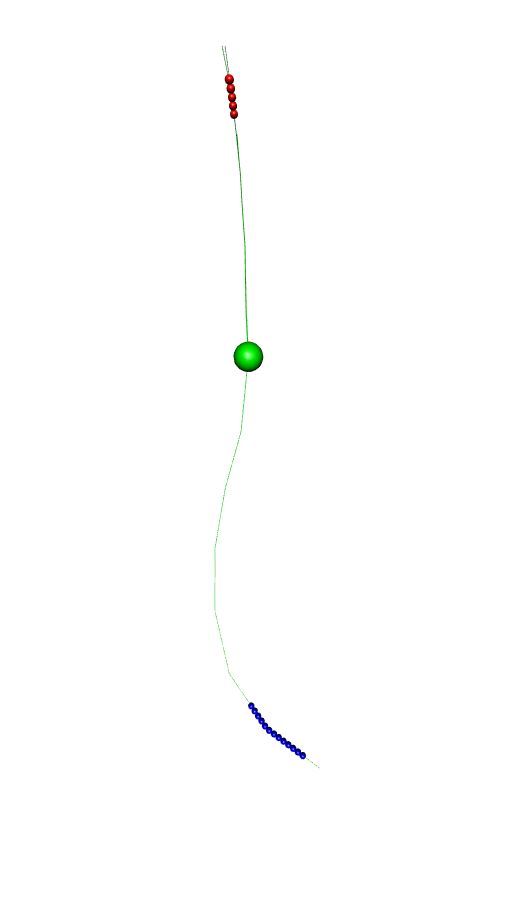
\includegraphics[width=0.7\columnwidth]{./Images_Result/rerative_sample.png}
         \caption{$BK\8&5f$N<jK!$G:n@.$7$??@7P:YK&7ABV(B}
         \label{Rerative_sampel}
       \end{subfigure}
       \caption{passive$B?@7P:YK&7A$NBVNc(B}
       \label{passive_morphos}
     \end{figure}

 \section{Ka$B%A%c%M%k$rMQ$$$?>l9g$N7k2L(B}
   $B?^(B\ref{Ka_Result1}$B$K(BKa$B%A%c%M%k$N$_$rF3F~$7$?:]$N7k2L$r<($9(B. $B?^Cf$N(BGausian$B$O%3%s%@%/%?%s%9J,I[$K(B
   $B%,%&%9J,I[$rMQ$$(B, $B%3%s%@%/%?%s%9J,I[(B

     \begin{figure}[H]
       \begin{subfigure}{0.5\columnwidth}
         \centering
         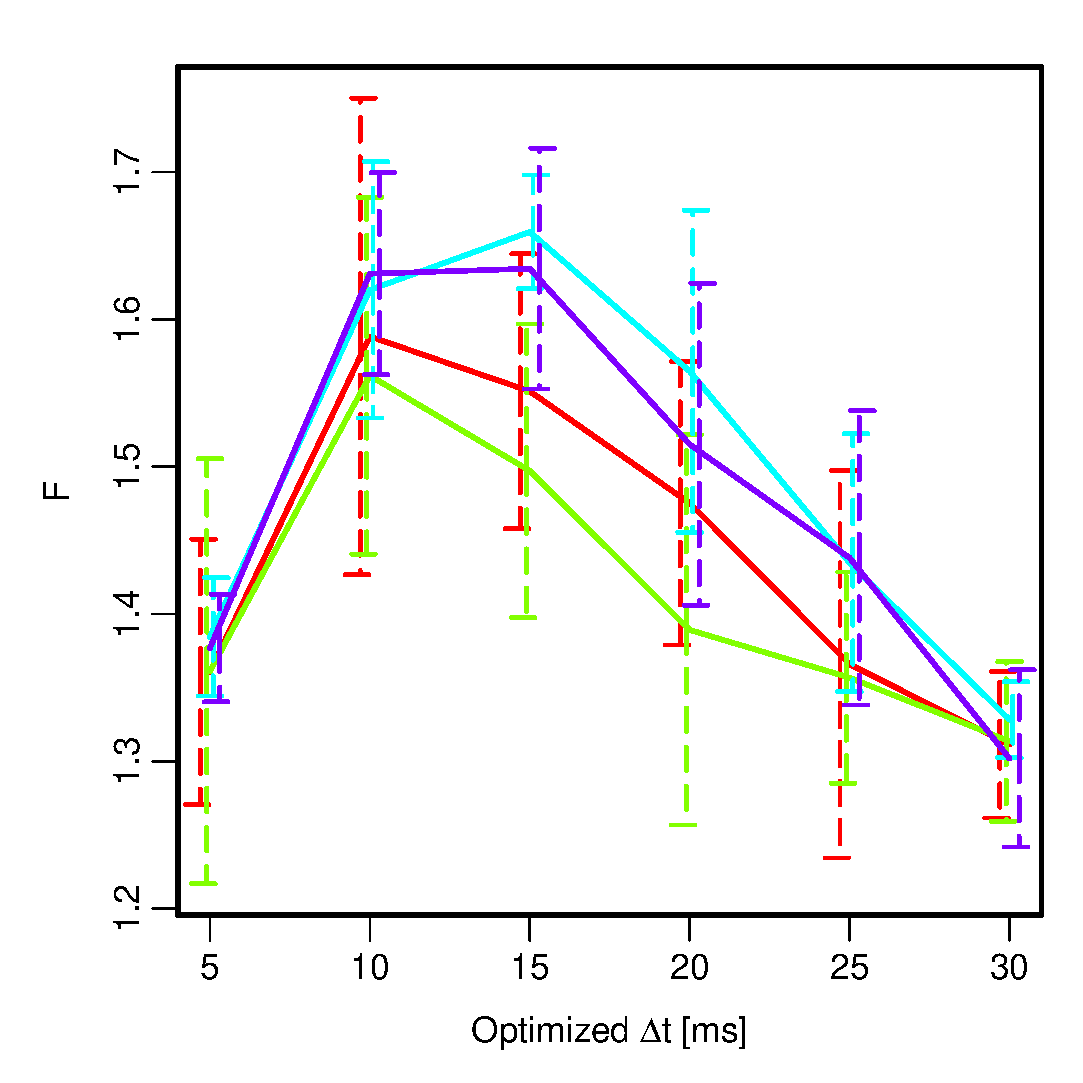
\includegraphics[width=0.8\columnwidth]{./Images_Result/k_test_F.eps}
         \caption{F}
         \label{k_5cells_F}
       \end{subfigure}
       \begin{subfigure}{0.5\columnwidth}
         \centering
         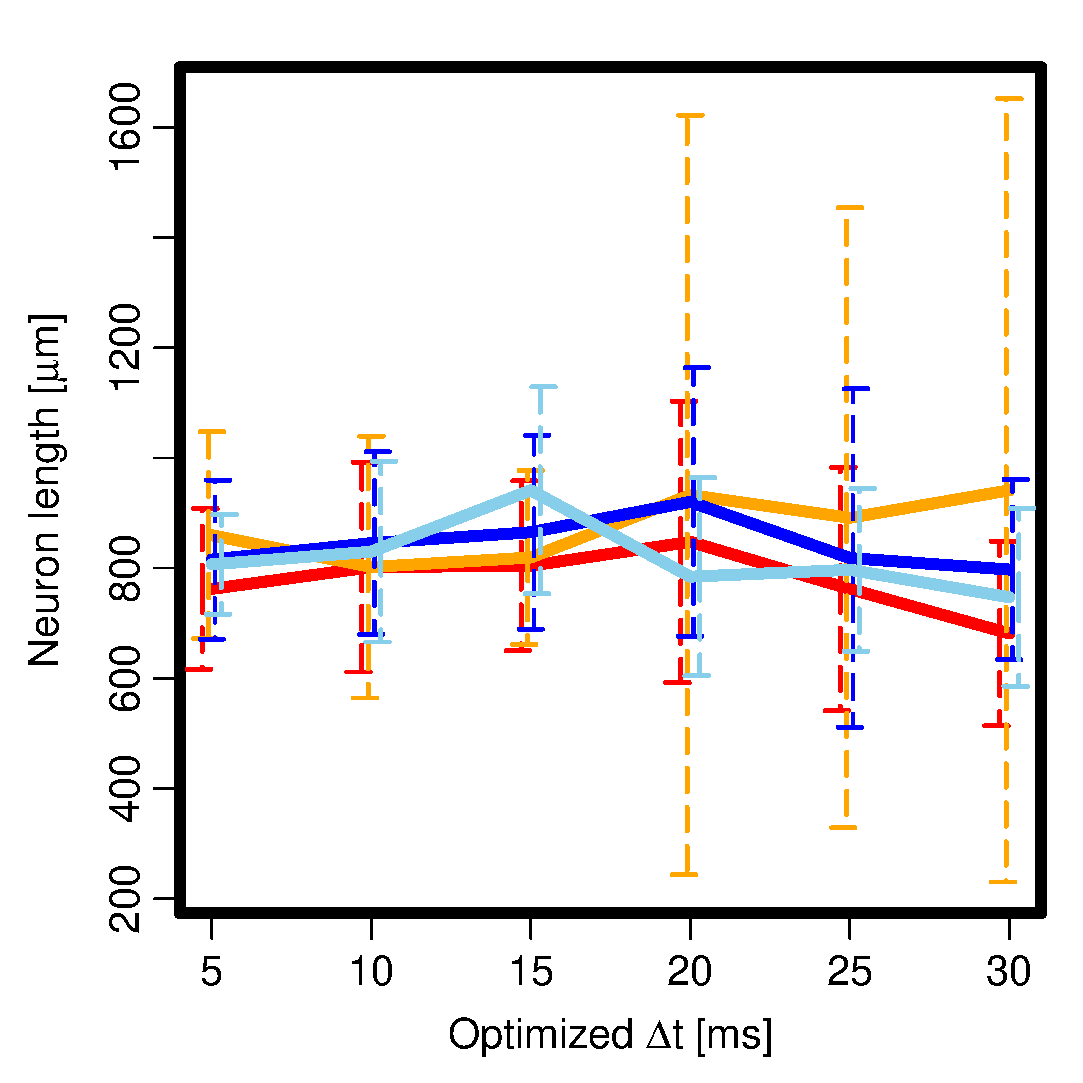
\includegraphics[width=0.8\columnwidth]{./Images_Result/k_test_TREE_length.eps} 
         \caption{$BD9$5(B}
         \label{k_test_TREE_length}
       \end{subfigure}

       \begin{subfigure}{0.5\columnwidth}
         \centering
         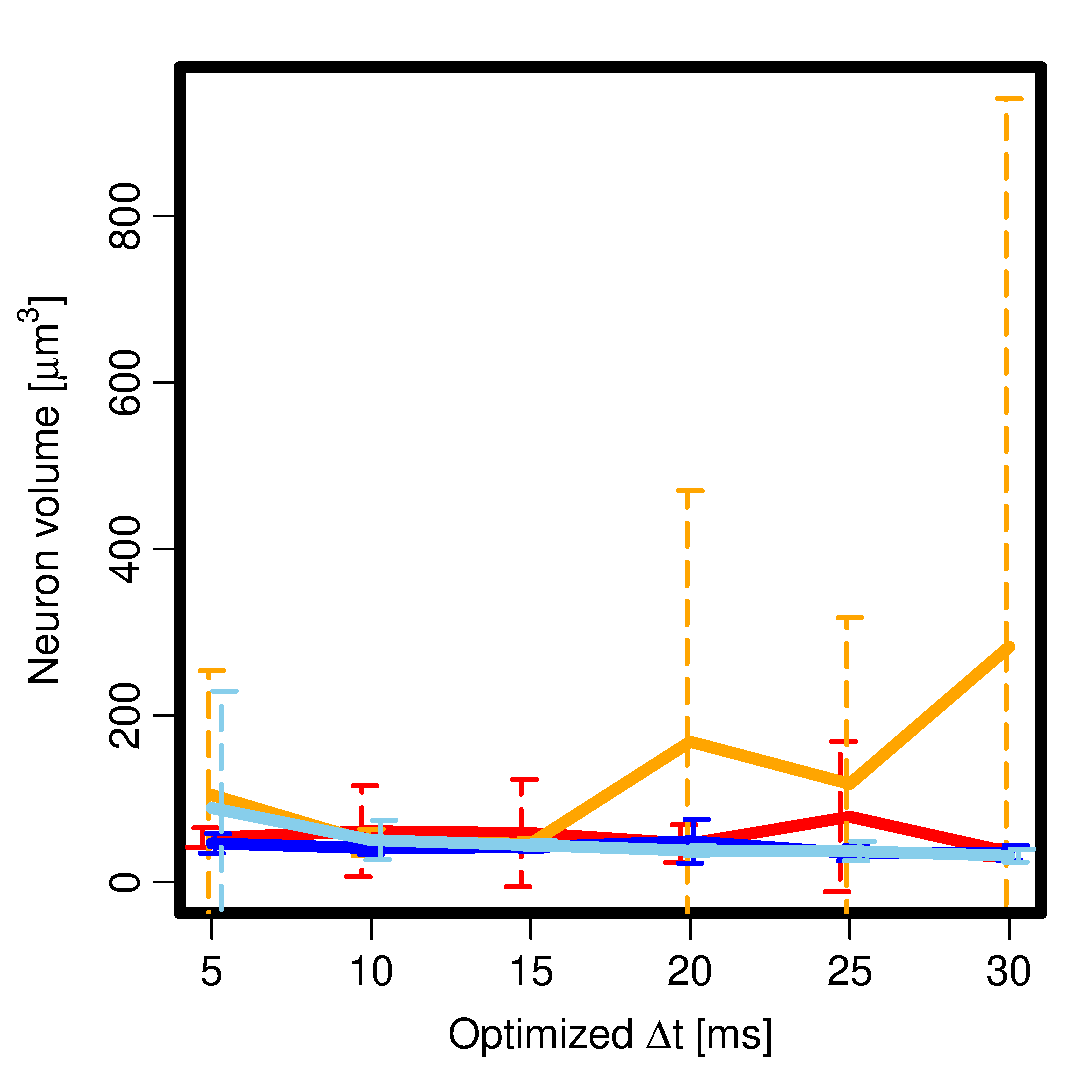
\includegraphics[width=0.8\columnwidth]{./Images_Result/k_test_TREE_volume.eps}
         \caption{$BBN@Q(B}
         \label{k_test_TREE_volume}
       \end{subfigure}
       \begin{subfigure}{0.3\columnwidth}
         \centering
         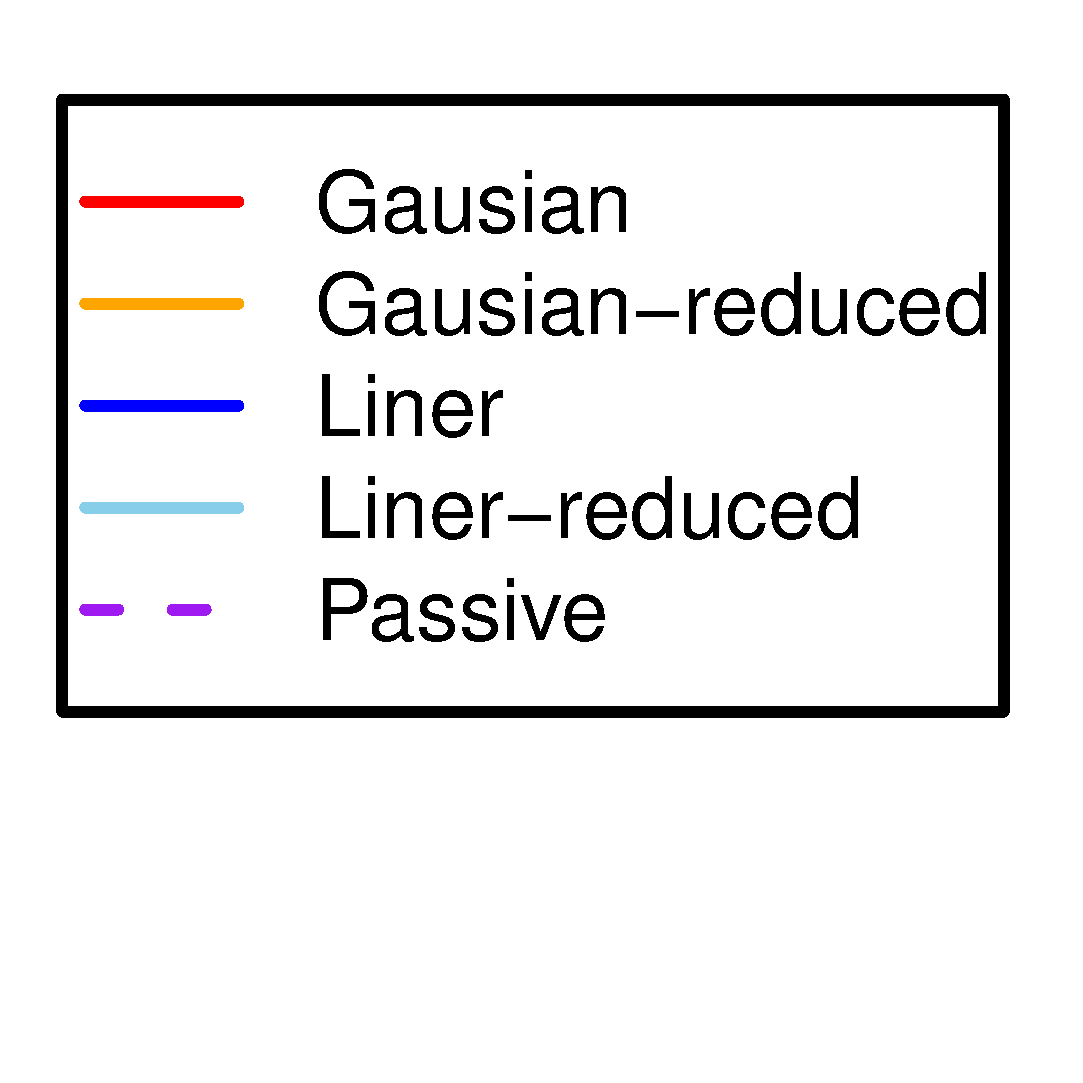
\includegraphics[width=\columnwidth]{./Images_Result/k_test_legend.eps} 
       \end{subfigure}
       \caption{Ka$B%A%c%M%k$rF3F~$7$?:]$N7k2L(B}
       \label{Ka_Result1}
     \end{figure}
 
 \section{CaT$B%A%c%M%k$rMQ$$$?>l9g$N7k2L(B}

 \section{Ka$B%A%c%M%k(B, CaT$B%A%c%M%k$rMQ$$$?>l9g$N7k2L(B}

